All experiments ran on the target machine (RTX 4090 Laptop GPU, 16\,GB VRAM; 64\,GB RAM; Windows~11; llama.cpp build b11620) with the \emph{real} local model, driven through the public HTTP API by \code{scripts/acceptance.py}, which records raw outcomes in \code{docs/ACCEPTANCE_RESULTS.md}. Unless stated otherwise the model was the \texttt{Q4\_K\_M} quantisation with a 16\,384-token context. Scenarios were run once each; this is a demonstration that the mechanisms work end to end, not a statistical estimate of success rates.

\subsubsection*{Acceptance scenarios}
Table~\ref{tab:acc} lists the seven scenarios and the independent evidence for each. \emph{All seven ended in a pass}, but three of them failed or crashed on earlier attempts for reasons described below; those attempts are retained in the raw results file rather than discarded.

\begin{table}[t]
\centering\small
\begin{tabularx}{\linewidth}{llX}
\toprule \textbf{Scenario} & \textbf{Outcome} & \textbf{Independent evidence}\\\midrule
Fix a failing test & pass & tests re-run by the harness after the agent finished: 2 passed; test file byte-identical to the original\\
Workspace boundaries & pass & requested absolute path outside the workspace was refused by the tool; file does not exist on disk\\
Git checkpoint restore & pass & after restoring the ``before'' checkpoint the original content was back and the newly created file was gone\\
Stop a running agent & pass & stop returned in 8.0\,s; task \textsc{cancelled}; no files written in the following 8\,s\\
Supervised approvals & pass (2nd run) & approved edit executed; denied command did not run; audit shows approved/denied per call\\
Restart and resume & pass & backend process killed with \code{taskkill /F} mid-task; recovered as \textsc{blocked}; resumed to \textsc{completed} with all three files\\
Full-stack app & pass & harness re-ran the agent's tests (10 passed) and exercised the live API (201/200/204)\\\bottomrule
\end{tabularx}
\caption{Real-model acceptance scenarios.}\label{tab:acc}
\end{table}

\paragraph{Fix a failing test.} The agent listed the directory, read the source and the test, and edited \code{calc.py} (\code{a - b} $\rightarrow$ \code{a + b}). Its first two \code{run_tests} calls failed because \code{pytest} was not installed in the global interpreter; the agent read the real error, installed it with \code{pip}, re-ran the tests (2 passed), recorded the fix in memory and finished. Nine model steps were used. The first failing runs are visible in the audit log, and the final report states ``Last test run: PASSED'' from that log.

\paragraph{Boundaries.} Asked to write a file at an absolute path outside the workspace, the model called \code{create_file}; the tool refused (``resolves outside the authorized workspace''). The model then tried a shell command, which requested approval and was denied by the harness, and finally created the file inside the workspace as the prompt allowed.

\paragraph{Supervised mode: a failed first attempt that taught something.} The first two runs of this scenario \emph{failed}. The command \code{echo hi > other.txt} was denied and recorded as denied, but the model then created \code{other.txt} with \code{create_file}, which also asked for approval --- and the test script approved every \code{create_file}. The enforcement worked as designed; the test was wrong, and the episode shows that a model \emph{will} try another route after a denial, so every route must pass the same gate. With the script corrected to approve only \code{notes.txt}, the audit log shows: \code{create_file} approved, \code{run_command} denied, \code{create_file} (for \code{other.txt}) denied, and \code{other.txt} did not exist.

\paragraph{Restart and resume.} After the first file was created, the back-end process was killed. A new process started with an empty memory; the task was recovered as \textsc{blocked} with the message ``Interrupted by application restart'', \emph{Resume} was invoked, and the model completed the remaining two files (8--9 steps in total over the two runs). The model call after resumption contained the pre-restart history and the interruption notice.

\subsubsection*{Full-stack application}
The prompt asked for a FastAPI + SQLite Todo application with a static JavaScript front end, a project-local virtual environment, pytest tests, and a live check in the browser. The Architect produced a plan of five milestones plus the automatic review. All seven tasks completed (Table~\ref{tab:fs}); the run used 142 tool calls, of which 14 returned errors that the agent then handled (for example a dev-server port already in use, and a mistaken selector in a browser test). The harness then verified the result \emph{without relying on the agent's report}: the agent's tests passed when re-run (10 passed), and a server started from the workspace answered \code{POST /api/todos} with 201, listed the new item, accepted \code{PATCH} (200) and \code{DELETE} (204), and served an HTML page that uses \code{fetch}.

\begin{table}[t]
\centering\small
\begin{tabular}{llr}
\toprule \textbf{Milestone} & \textbf{Role} & \textbf{Model steps}\\\midrule
Plan: architecture and task breakdown & architect & 3\\
Scaffold project (venv, requirements) & developer & 8\\
Implement FastAPI backend & developer & 30\\
Create static front end & developer & 37\\
Write and run pytest tests & developer & 6\\
Runtime verification in the browser & tester & 19\\
Final review & reviewer & 6\\\bottomrule
\end{tabular}
\caption{Full-stack run: milestones and model steps (Q4\_K\_M).}\label{tab:fs}
\end{table}

\paragraph{This was not a clean run, and we report it as it happened.} The elapsed time of about eight hours is \emph{not} a performance figure. (The harness printed 553 minutes; that number was inflated by a timestamp bug, described in Section~\ref{sec:lessons}, which made browsers and scripts read UTC times as local time.) The elapsed time includes (i) two stalls, of the order of twenty minutes each, in which the agent sat waiting for an approval that the test script was not written to answer --- caused by a classifier false positive on a harmless \code{python -c "...; print(...)"} command (Section~\ref{sec:lessons}) --- one of which a human approved, after which the classifier was fixed in code; (ii) a back-end restart followed by a \emph{Resume} of the same task, which worked; (iii) periods when a second client (the Cline editor extension) was using the same single model and slowed both, from about 7 to about 2.5 tokens/s; and (iv) the test script's own timeouts. Dev servers started by the agent also survived the back-end restart and kept their ports, which made a later \code{start_dev_server} fail with ``port in use''; the agent worked around it, and we list this as a limitation.

\subsection{Quantisation trade-offs: speed, memory and quality}\label{sec:quant}
The 15.4\,GiB \texttt{Q4\_K\_M} file does not fit in 16\,GB of VRAM together with the KV cache, so llama.cpp runs some layers on the CPU. We therefore measured two smaller quantisations of the same model under identical conditions (context 65\,536, KV cache \texttt{q8\_0}, flash attention, one request at a time, nothing else using the GPU): \texttt{IQ4\_XS} (13.4\,GB) and \texttt{IQ3\_S} (11.1\,GB). Each model received the same fixed workload: a 400-token generation, an 7\,318-token prompt, six tool-calling cases with exact expected arguments, and eight coding tasks whose answers were \emph{executed} against hidden tests (the tests were first validated against reference solutions, and a deliberately wrong solution was confirmed to fail). Table~\ref{tab:quant} and Figure~\ref{fig:speed} show the results.

\begin{table}[t]
\centering\small
\begin{tabular}{lrrr}
\toprule & \textbf{Q4\_K\_M} & \textbf{IQ4\_XS} & \textbf{IQ3\_S}\\\midrule
File size (GB) & 15.41 & 13.41 & 11.13\\
VRAM in use (GB) & 13.7 & 13.7 & 13.3\\
Generation (tokens/s) & 7.2 & 9.5 & \textbf{35.9}\\
Prompt processing (tokens/s) & 584 & 677 & \textbf{1195}\\
GPU utilisation (\%) & 30 & 34 & \textbf{94}\\
CPU cores busy (of 32) & 20 & 21 & \textbf{1}\\
Tool calls correct & 6/6 & 6/6 & 6/6\\
Coding tasks passed & 7/8 & 6/8 & 7/8\\
Mean time per coding task (s) & 184 & 137 & \textbf{47}\\\bottomrule
\end{tabular}
\caption{Same model, three quantisations, identical workload (measured). VRAM figures are the whole-GPU reading while the server was busy.}\label{tab:quant}
\end{table}

\begin{figure}[t]
\centering
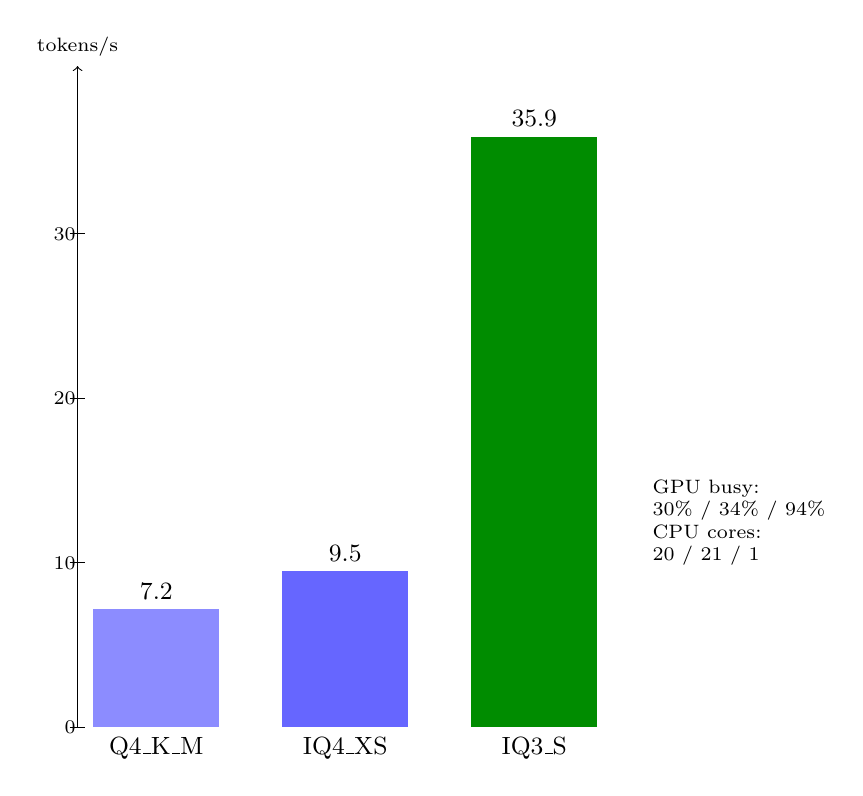
\begin{tikzpicture}[x=1cm,y=1cm,font=\small]
  \def\h{0.095}
  \foreach \name/\v/\c/\x in {Q4\_K\_M/7.2/blue!45/0, IQ4\_XS/9.5/blue!60/2.4, IQ3\_S/35.9/green!55!black/4.8}{
    \fill[\c] (\x,0) rectangle (\x+1.6,\v*\h*2.2);
    \node[above] at (\x+0.8,\v*\h*2.2) {\v};
    \node[below] at (\x+0.8,0) {\name};
  }
  \draw[->] (-0.2,0)--(-0.2,8.4) node[above,font=\scriptsize]{tokens/s};
  \foreach \t in {0,10,20,30}{\draw (-0.3,\t*0.209)--(-0.1,\t*0.209) node[left,font=\scriptsize]{\t};}
  \node[font=\scriptsize,align=left] at (8.2,2.6) {GPU busy:\\30\% / 34\% / 94\%\\CPU cores:\\20 / 21 / 1};
\end{tikzpicture}
\caption{Generation speed in tokens per second (bars drawn to scale). Only IQ3\_S fits entirely in VRAM, which is why the GPU is busy and the CPU idle.}\label{fig:speed}
\end{figure}

\paragraph{Reading the numbers.} Speed is governed by \emph{where the weights live}, not by arithmetic precision alone. With the two larger files part of the model runs on the CPU, so each token waits on the slower processor while the GPU idles (30--34\,\% busy, about 20 CPU cores saturated). \texttt{IQ3\_S} fits completely in VRAM: the GPU is 94\,\% busy, one CPU core is used, and generation is about five times faster. The same effect explains why the dedicated GPU appeared ``not busy'' during the agent runs above.

\paragraph{Quality.} On this small workload the three quantisations were indistinguishable in tool-call reliability (all 6/6) and within one task in coding (7/8, 6/8, 7/8). All three failed the same task, \code{parse_csv_line}, and in every case the recorded finish reason was \code{length}: the model's reasoning consumed the entire 6\,000-token limit before any code was emitted, so the failure reflects the token cap and the long reasoning of this model family, not wrong code. The single genuine logic error was by \texttt{IQ4\_XS} on \code{LRUCache} (a helper class referenced without \code{self.}); the other two solved it. One extra miss in eight tasks is within what chance could produce, and \emph{we draw no conclusion that \texttt{IQ3\_S} is as good as \texttt{Q4\_K\_M} in general}.

\paragraph{Threats to validity.} Eight short tasks, one run each, temperature 0.2, one machine; the tasks are small functions, not repository-scale changes; the full-stack acceptance run used \texttt{Q4\_K\_M} only; and lower-precision quantisations may degrade more on long, multi-step work than these tests can reveal. The practical recommendation that follows is to use \texttt{IQ3\_S} for interactive work where latency dominates and keep \texttt{Q4\_K\_M} available for hard tasks, verifying with the test suite either way.
